\documentclass[ letterpaper, 10 pt, conference]{ieeeconf}  % Comment this line out if you need a4paper

\IEEEoverridecommandlockouts                        
\overrideIEEEmargins                                      % Needed to meet printer requirements.



\usepackage{booktabs}
\usepackage{graphicx}
\usepackage{cite}
\usepackage{url}
\usepackage{algorithm}
\usepackage{algorithmic}
\usepackage{amsmath}
\usepackage{caption}
\usepackage{subcaption}
\usepackage{units}

%\usepackage{appendix}


\usepackage{wrapfig} % Wraps text round images

\usepackage{epstopdf}

\newtheorem{definition}{Definition} 

\DeclareMathOperator{\diff}{diff}
\DeclareMathOperator{\adv}{adv}
\DeclareMathOperator{\card}{card}



\title{\LARGE \bf
%Illustration of the shortcomings of control based plume tracking approach using a dynamic plume simulation. 
Dynamic Modeling and Simulation of Ocean Pollution Plumes for Robotic Control Design}


\author{Nathaniel Saul$^{1}$, John Marriott$^{1}$, Brian Bingham$^{2}$, Muhammad Fahad$^{3}$,  and Yi Guo$^{3}$ % <-this % stops a space
\thanks{$^{1}$Nathaniel Saul and John Marriott are with the Department of Mathematics, University of Hawaii at Manoa, Honolulu, HI 96822, USA {\tt\small sauln@hawaii.edu, marriot@math.hawaii.edu }}%
\thanks{$^{2}$Brian Bingham is with the Department of Mechanical Engineering, University of Hawaii at Manoa,
        Honolulu, HI 96822, USA {\tt\small bsb@hawaii.edu}}%
\thanks{$^{3}$Muhammad Fahad and Yi Guo are with Department of Electrical \& Computer Engineering Stevens Institute of Technology, Hoboken, NJ 07030, USA.  {\tt\small mfahad@stevens.edu, yguo1@stevens.edu}}%
}


%%%%%%%%%%%%%%%%%%%%%%%%%%%%%%%%%%%%%%%%%%%%%%%%%%%%%%%%%%%%%%%%%%%%%%%%
%These are all packages that I have added
\usepackage{amsmath}
\newcommand\numberthis{\addtocounter{equation}{1}\tag{\theequation}}
\usepackage{cite}

\usepackage{listings}    
\usepackage{hyperref}
%%%%%%%%%%%%%%%%%%%%%%%%%%%%%%%%%%%%%%%%%%%%%%%%%%%%%%%%%%%%%%%%%%%%%%%%%%


%\%title{Plume Simulation}
%\author{Nathaniel Saul, Muhammed Fahad, Brian Bingham, Yi Guo}

\begin{document}
\maketitle
\thispagestyle{empty}
\pagestyle{empty}



%%%%%%%%%%%%%%%%%%%%%%%%%%%%%%%%%%%%%%%%%%%%%%%%%

\begin{abstract}

We present a model of the dynamics of an ocean pollution plume developed specifically for evaluating the performance and stability of robotic command and control algorithms. The key feature of our model is the ability to represent temporal and spatial sparsity as a model parameter.  This approach provides a quantifiable, metric-based method for evaluating the affect of chemical concentration intermittency on the performance and stability of autonomous robot control algorithms.

%relationship between the performance and stability of robotic control algorithms with respect to the sparsity of plume dynamics and the intermittency of the sensor observations.   
\end{abstract}
%\tableofcontents
%We showed that as it stands, the control algorithm based solely on a time-averaged plume model does not work in more complicated situations, and it is not expected to work in application.  To do this, we generated a oil spill model that captures many of the instantaneous spatial and temporal characteristics of dynamic plumes.  With simulation, we show that controller fails.  We describe what is wrong with the algorithm and suggest ways to improve upon it


%%%%%%%%%%%%%%%%%%%%%%%%%%%%%%%%%%%%%%%%%%%%%%%%%%%%%
%%%%%%%%%%%%%%%%%%%%%%%%%%%%%%%%%%%%%%%%%%%%%%%%%%%%%

\section{Introduction}

The study of plume models originated with early research to understand the dynamics of smoke rising from a chimney \cite{Bosanquet1936}.  Over the $20^{th}$ century, research has expanded to better understand the temporal and spatial distribution of chemical concentration outflows in a variety of fluid environments. The environmental representation we propose is based upon coastal ocean models which has been thoroughly studied by the oceanographic community.  In this work we adapt these standard models to provide predictions of chemical concentrations that would be observed by autonomous marine robots operating in proximity of a pollution source.  The purpose of this effort is to develop a virtual environment for evaluating heterogeneous teams of marine robots tasked with characterizing point-source pollution sources such as hydrocarbon spills and leaks; however, the model we propose is sufficiently general to capture the salient dynamics of a variety of pollution scenarios.  

%This paper models the dynamics of oil spills, which is a growing concern with the increase in off-shore oil-rigs and global transport of oil.  The results of an oil spill can be catastrophic.  For damage mitigation and clean-up many research communities have turned their eye to the field of robotics.  
%The plumes that are of particular interest in this paper are those of accidental dumping of oil in water, or more generally, oil-spills.  

A critical aspect of the proposed environmental model is its ability to represent temporal and spatial variability as a parameter of the model.  With sufficient averaging in time and space the distribution of chemical agents introduced in the marine environment can be considered to be smoothly distributed based on advection, diffusion, and dissolution.  In such an idealized environment control algorithms can make use of observations of smooth gradients to achieve their particular goal, e.g., localizing the pollution source or following the plume front.  However, previous studies on chemical plume tracking \cite{pang06chemical,Jones1983}  have demonstrated that the point measurements in such an environment are intermittent, suggesting significant temporal and spatial variability.  These chemical \emph{packets} or \emph{filaments} lead to steep localized gradient observations from mobile platforms, particularly in turbulent environments.  Control strategies for multi-robot teams to characterize such environments must be robust with respect to this variability.  Therefore the modeling approach we present includes an overt representation of this variability to enable quantifying the robustness of candidate control strategies.


%The most critical part of robotic systems is the command and control algorithms,  which determine how the robots manoeuvre around and in the oil spill and complete their objective.   Many control algorithms are robust enough that when generated using a simplified world model they easily succeed in real application.  Others are fragile and easily break if the model they are developed from is not perfect.  

Our research group previously proposed a controller to use with multiple heterogeneous robots to track and monitor an oil spill \cite{Li2014}.   The controller is a modified gradient descent which enables the robot to follow the plume front, mapping the extent of the plume as it evolves over time.
%moves the robot along edge of the plume and follows the plume front to map the extent of the plume as it evolves in time.  
By testing this control approach with the model presented below we are able to analyze the robustness of such a multi-robot control algorithm to the sparsity of field observations.  Furthermore we illustrate quantifying control performance with respect to the variability associated with plumes that exhibit the packet or filament type distributions as expected in field operations.

This paper will present a model that can capture both the time-averaged, idealized structure as well as the instantaneous, realistic structure of a dynamic plume as measured by on-board robot sensors.  We describe two defining metrics of an instantaneous plume---the concentration sparsity and concentration peak/mean ratio---and show how to simulate the change from ideal plume to realistic plume by adjusting a single parameter of the model implementation. This method of emulating a pollution plume enables evaluation of the robustness of autonomous robotic sampling strategies with respect to observed variability; the proof-of-concept implementation of the Li et al. approach \cite{Li2014} is used to demonstrate this capability.  For this illustrative test case we confirm the control approach performs well for when variability is low, the idealized case, and that the performance degrades as the variability increases.  Furthermore we analyze how the performance degrades as a function of observation variability.

Section \ref{part:background} of this paper details the plume characteristics most important for our use and briefly reviews the basic methods of modeling these characteristics. 
Section \ref{part:relatedWork} describes other plume models in prominent use and compares their usefulness with respect to our objectives.
Section \ref{part:implementation} presents our proposed model as well as the specific implementation.  Section \ref{part:tuning} illustrates how the implemented model can capture both time-averaged and instantaneous characteristics of plumes and can be used to test robotic controllers.  
Section \ref{part:caseStudy} presents a case study were the environmental model is used to evaluate the controller proposed by Li et al. \cite{Li2014}.


%A second paper will apply the model presented here to evaluate multi-robot command and control approaches.  We will report on the application of this model to the development and evaluation of multi-robot control approaches to the problem of characterizing pollution plumes in a coastal environment.


\section{Background and Related Work}
\subsection{Fundamentals of Plume Modeling} \label{part:background}
%\section{Background}

%Some of these focus on modelling plumes in the atmosphere and some focus on modelling oil-spills.  
Models have been developed for plumes in many different environments: atmosphere, water surface, and deep water for example.  Over fifty different models specific to oil spills have been developed. Of these, a handful are still widely used \cite{ASCE1996}.   The focus of this paper is models of ocean pollution that capture the temporal and spatial concentration evolution at the air-sea boundary.  The dominant components of such models are advection (transfer of pollution by ocean current) and turbulent diffusion (transfer of pollution due to concentration gradients and shear flow). Secondary effects also play a role:  evaporation, molecular diffusion, dispersion, emulsification, and interactions with ice and shore. 

Evaporation can be an important component when volatile pollutants %dominate when 
first reach the water surface and becomes less of an issue later when most of the materials have evaporated.  Emulsification is the breakdown of large heterogeneous globules of pollutant into smaller uniform globules.  
Molecular diffusion is diffusion as a result of molecular properties particular to the pollutant.  
Interaction with the shore and ice is relevant only when the polluting event is near the coast or in the Arctic.
Many of these models do not significantly effect the two metrics---sparsity and peak/mean ratio--- or are only relevant in specific situations, such as when the considering cases near floating ice.  


Plumes are often generalized as having smooth gradients where the concentration follows a normal curve.  This generalization is a time-averaged representation of the concentration and location, usually of three minutes or longer \cite{Jones1983}.  The Gaussian model, based on partial differential equations, is explicitly designed to model the time-averaged plume \cite{Elkinton1984}.  The defining equation for the Gaussian plume model is
	\begin{equation}\label{eq:OrigPlume}
	\frac{\partial c(x,t)}{\partial t} + v^{T}(x,t)\cdot \nabla c(x,t) = D\nabla^2 c(x,t)
	\end{equation}
where $v$ is the velocity vector of the environment flow, $\nabla c(x,t)$ is the concentration gradient, $\nabla^2 c(x,t)$ is the concentration divergence at point $x$ and time $t$ and $D$ is a diffusion coefficient of the material.

The Gaussian model is the oldest of the plume modeling techniques and is used extensively to model atmospheric plumes. Because the Gaussian is a time-averaged model, it idealizes some of the more interesting characteristics a plume can have, specifically, the features of an instantaneous plume. 

We use two main metrics to quantify the instantaneous characteristics of a plume:  the sparsity and the peak/mean ratio. 

\begin{definition}[Sparsity]
The sparsity is defined as the percentage of concentration readings in a stationary point over a certain threshold as a plume migrates over that point.  
\end{definition}


Sparsity is calculated as the cardinality of the set of concentration readings at a point under a defined threshold,  over the cardinality of the set of all samplings at the same point. Sparsity can be modeled as 
\begin{equation}
T_x = \{t \in S_x | \ t> \theta \}
\end{equation}
\begin{equation}
\mbox{sparsity} := \frac{|T_x|}{|S_x|}\\
\end{equation}
where $S_x$ is the set of all recent samples and $T_x$ is the set of all samples above a threshold $\theta$\cite{Jones1983}.


\begin{definition}[Peak/mean ratio]
The peak/mean ratio is defined as the ratio between the peak concentration value and the time-averaged mean of concentration at a stationary point as a plume migrates over that point,
\begin{equation}
\mbox{peak/mean ratio} := \max(S_x)/\frac{1}{|S_x|}\sum{S_x}.
\end{equation}
where $\max(S_x)$ is the maximum concentration reading in the set of recent samples, $S_x$, and $\frac{1}{|S_x|}\sum{S_x}$ is the mean concentration reading across the same set of samples \cite{Crimaldi2002}.

\end{definition}


Jones showed that for some kinds of plumes, the sparsity at any given location can be upwards of 90\% \cite{Jones1983}.  That is, for 90\% of the time, a stationary sensor will read zero (or below a sensing threshold) as the plume moves through the point.   A study by Crimaldi et al. found that peak concentration can be three orders of magnitude larger than the mean \cite{Crimaldi2002}. These metrics are shown qualitatively in Fig.~\ref{pic:simSpont}.  This figure was generated using the simulation described below and will be used to compare the validity of our model with the metrics defined by Jones and Crimaldi.  Notice the peak over $50$ samples is normalized to $1$ and the mean is almost exactly $1/3$.   Qualitatively, the majority of the readings are below the mean. 

\begin{figure}[thpb]
      \centering	
	\framebox{\parbox{3in}{
	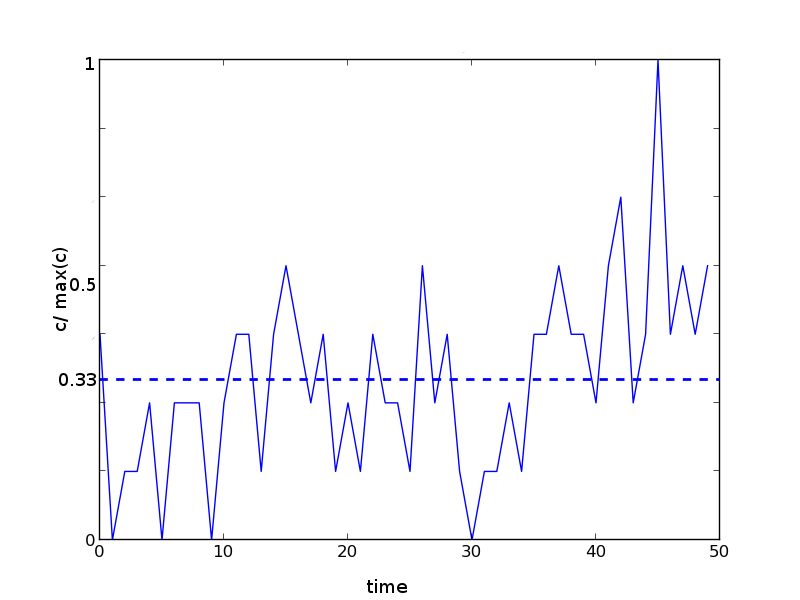
\includegraphics[width=3in]{../plots/inUse/normedExample.png}}}
      \caption{The Simulation sparsity snapshot}
      \label{pic:simSpont}
 \end{figure}

Since the instantaneous concentrations are of great concern for robots navigating a plume,  the Gaussian model alone is not sufficient to test control algorithms that rely on instantaneous, fine scale readings of a plume.    


The Lagrangian method is a particle based model that depicts the plume as  an aggregate of many individual particles, each moving according to the advection laws and a random walk derived from the Gaussian equations.   In the limit, as the number of particles approaches infinity and the time step approaches zero, the Lagrangian model approaches the Gaussian model, but when it is far from the limit, the Lagrangian model has the structure very similar to the sparse metrics described by Jones and Crimaldi.  As a result, this method  much more capable of representing the instantaneous dynamics of a plume.


%The Lagrangian is derived from the Gaussian, at the limit it is the Gaussian.  This model can also be much more variable. far from the limit, it can portray some of these instant characteristics.  

The generic defining equation for the Lagrangian random walk method is
	\begin{equation}\label{eq:Lagrange}
	x_i(t+ \Delta t) =x_i(t) +  \adv{(t, x_i(t),  \Delta t )} + \diff{(t, x_i(t), \Delta t)}  
	\end{equation}
where $x_i(t)$ is the location of the $i^{th}$ particle at time $t$, $\Delta t$ is the time step, $\adv{(t,x(t), \Delta t)}$ is the advection component and $\diff{(t, x(t), \Delta t)}$ is the diffusion component of the particle movement.  Many different ways to model the advection and diffusion equations exist. Usually advection is determined by the velocity vector of the fluid field at location $x(t)$ and time $t$ and the diffusion is a function of the diffusion coefficient for the material and a random variable.    Many other higher order and situational effects can be modeled using the Lagrangian method by superposing their contribution to the particle movement or periodically removing individual particles from the map. 

\subsection{Related work}\label{part:relatedWork}

%\subsubsection{Oil-fate modeling}

The Lagrangian model is now the dominant model used for studies the dynamics of marine pollution.  Such fate models focus on the distribution of the pollutant after a certain amount of time. These models use location specific environmental data for currents and wind.  Many derivations of the Lagrangian model have been proposed and implemented  \cite{ASCE1996}.  


%these 2 paragraphs can probably get cut out:
The General NOAA Operational Modeling Environment (GNOME) is a widely accepted tool produced and verified by NOAA \cite{GNOME}.  This software tool uses historical weather data to model the fate of the oil spill.  GNOME can be very useful for simulating the transport and fate of oil spills in specific places around the world.  It comes equipped with historical current and wind data and can simulate oil spills of many different kinds of oil. 
The main concern with the GNOME software is that the step size (15 minutes) is on a scale much too large to accurately reflect the instantaneous dynamics of a plume necessary for evaluating robotic remediation strategies.  A European model MEDSLICK provides detailed simulation of oil spills very similar to GNOME \cite{Dominicis2013} \cite{Dominicis2013a}. It suffers from the same problem as GNOME of using a time and space scale much too large for testing of robotic response.  

Researchers have tackled the problem of understanding and containing oil-spills from a number of different perspectives.  In the robotics community, researchers study source localization, edge tracking, and autonomous clean-up, with single and multiple robots.  Those who study plume source localization generally base their approach on biomimetic techniques, trying to understand and emulate how animals find plume sources \cite{Farrell2003}\cite{Li2006}\cite{Webster2001a}.  Other strategies focus on the problem by looking at optimal ways to lay out robotic sensor networks for spill tracking and monitoring of the plume edge \cite{Grasso2001}\cite{Li2014}\cite{Zhang2007}\cite{Sahyoun2010}.  Some strategies specifically focus on robotic clean-up and how to generate complete mapping of the dynamic plume \cite{Jin2014}\cite{Zarzhitsky2005}, and spill finding \cite{Marjovi2014}.  Additionally, many of the techniques have been developed for individual and multiple robots \cite{Grasso2001}\cite{Li2014}\cite{Marjovi2014} \cite{Zarzhitsky2005}.   

Theoretical development of the above techniques usually use either the Gaussian or Lagrangian model for simulation.   Marjovi and Marques use a Gaussian plume model for development of their algorithms for swarm odor plume finding \cite{Marjovi2014}.  Sahyoun et al. also use a Gaussian plume model to develop algorithms for plume tracking with mobile sensors \cite{Sahyoun2010}.  

Farrell et al. have attempted to capture the instantaneous structure of plume behavior using a variation of the Lagrangian method \cite{Farrell2002} \cite{Farrell2003}.  This approach simulation is suited for capturing the instantaneous dynamics of an odor plume and has led to control strategies that emulate how moths find the source of an odor plume \cite{Farrell2002}.  A similar model is used by Li et al. to test source localization algorithms based on moth behavior \cite{Farrell2003} \cite{Li2006}.  Zarzhitsky et al. also used the model developed by Farrell to simulate swarm chemical plume tracing \cite{Farrell2002}\cite{Zarzhitsky2005} .  This model is not applicable to oil spills because it does not model large-scale turbulence and thus presents a largely laminar plume.  Though it emulates the sparse metrics described by Jones and Crimaldi, it is incapable of also emulating the idealized plume described by the Gaussian equations.


\section{Plume Model and Simulation} \label{part:implementation}
\subsection{Model Implementation}
Many models for the advection and diffusion component of the Lagrangian method exist.   In this paper we use an adaptation of the equations derived by Chao and verified experimentally by Nagheeby et al. \cite{Chao2003} \cite{Nagheeby2010}.   This model accounts for many effects on the plume besides advection and diffusion, such as evaporation, dissolution, shoreline and ice interaction,  and emulsification.  In the interest of brevity, the examples we discuss below are constructed for a scenario where advection and diffusion are dominate.


%All of these but advection and diffusion can be ignored for this simulation as they do not play a significant role in the time scale we are interested in or do not significantly effect the specific plume characteristics we are interested in.  

We implemented the Lagrangian model \eqref{eq:Lagrange} in the paper with the $x$ and $y$ components of the advection and diffusion components are as follows.  Eqs. \eqref{YapaChao}-\eqref{chaoEnd} show the advection and diffusion the equations used in this simulation,   

\begin{align}
\adv_x{(x,t)}  &=k_t u_x + k_w w_x \label{YapaChao} \\
\adv_y{(x,t)} &=k_t u_y + k_w w_y \\		
\diff_x{(x,t)}  &= R_1  \left(12 D \Delta t \right)^{1/2}\cos(2\pi R_2) \label{dif3}\\
\diff_y{(x,t)}  &= R_3  \left(12 D \Delta t \right)^{1/2}\sin(2\pi R_4) \label{chaoEnd}
\end{align}
where $u$ and $w$ are the current and wind vectors respectively, $k_t$ and $k_w$ are constants used to capture the impact of the current and wind.  Chao recommends these be set to $1$ and $0.03$ respectively.  $R_i$ is a unique uniform random variable on the interval $[0,1]$.   $D$ is the diffusion coefficient, typically set between $0.01\  \mbox{m}^2/\mbox{s}$ and $0.5\ \mbox{m}^2/\mbox{s}$.

We implemented the above model in Python as a standalone process.  This allowed us to use the real-time control software processes by having the environmental module pass simulated sensor measurements to the controller via inter-process communication.  The message passing between processes is implemented using the Lightweight Communications and Marshalling (LCM) library\cite{Huang2010}.  This work flow enables rapid transition between controller development (in offline and real-time simulation) and field deployment on sensor-equipped mobile robotic platforms (real-time control).

Fig. \ref{pic:framesByTime} shows an example of the simulated plume evolution.  This density histogram shows the results of the plume emitted from a source located at $(12,26)$ at $2, 5, 8$, and $11$ hours after the pollution begins. 
\begin{figure}[thpb]
      \centering
	\framebox{\parbox{3in}{
	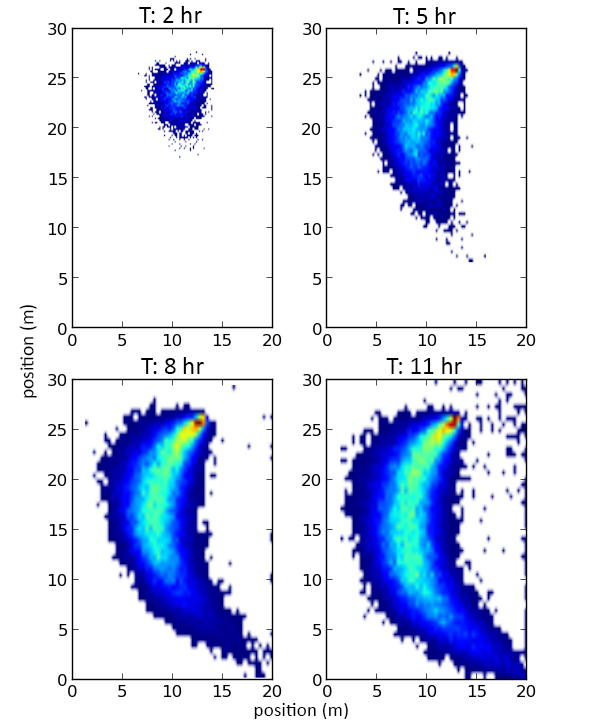
\includegraphics[width=3.2in]{../plots/newUse/timeFrameslabel.png} } }
      \caption{Two-dimensional histogram of plume concentration at 2, 5, 8, and 11 hours after release}
   \label{pic:framesByTime}
 \end{figure}
%\subsection{Concentration Calculations}

Calculating the concentration is done by counting all of the particles within a certain radius from the point in question,
	\begin{equation}\label{eq:concentration}
	c(x,t) =  \card({\{m | m \in B(x,r)\}}) 
	\end{equation}
where the concentration at location $x$ and time $t$ is the cardinality of the subset of particles inside a ball centered at $x$ with radius $r$, $B(x,r)$.   For our implementation, we chose the ball using the $L_{\infty}$ norm.  %The count is then multiplied by a normalizing factor $n$:
%\begin{equation} \label{eq:normalizer}
%n =  \sigma/A.  
%\end{equation}
%I don't really like how this normalize factor is used.  It's kind of artificially contrived.  
%based on the area of the ball, $A$, and the density of each particle, $\sigma$. 



\subsection{Parameterizing Intermittency}\label{part:tuning}

We consider the time-averaged plume and the instantaneous plume as two extremes of what our plume model should be capable of simulating.  On one hand, the smooth gradients are completely idealized;  on the other hand, the instantaneous plume is extremely sporadic and irregular.   
%%%%reword me
The simplicity of the Lagrangian method modeling the plume as composite of many individual particles allows the model to reach near the Gaussian time averaged plume and near the instantaneous plume, and everywhere in between.    %%up to here-  shoot for succinct and formal
Also, the Lagrangian model uses a moving frame of reference, and thus only calculates the concentration of a point based on the particles that are nearest that point, no interpolation and smoothing between gridded blocks occurs in the simulation.  This allows for the simulation to produce extremely varying fluctuations in concentration readings over both space and time \cite{Crimaldi2002} \cite{Jones1983} \cite{Webster2001} .  


%this image can probably also go. 
\begin{figure}[thpb]
      \centering

	\framebox{\parbox{3in}{
		%\framebox{\parbox{1.3in}{
		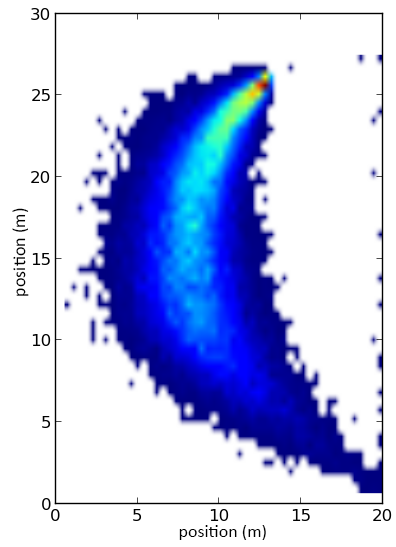
\includegraphics[width=1.5in]{../plots/newUse/snapShotTrim8l.png}%}%}%\framebox{\parbox{1.3in}{
		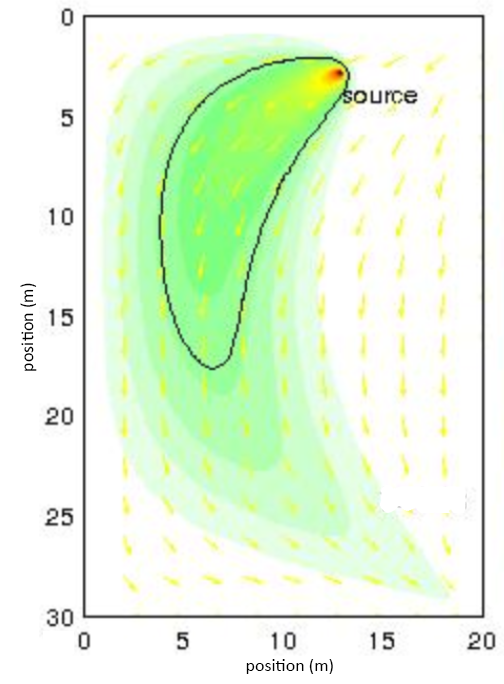
\includegraphics[width=1.5in]{../plots/newUse/shuaiShotlabelpng.png}
		%}}
	}}
      \caption{The Lagrangian model on the left compared with the Gaussian model on the right}
      \label{pic:tuneUp}
 \end{figure}

In the limit, as the time step approaches zero and the number of particles approaches infinity, the model approaches the Gaussian model.   Fig. \ref{pic:tuneUp} shows a concentration map of the Lagrangian particle plume generated in this study side-by-side with the Gaussian model originally used to develop the controller under study \cite{Li2014}.  This shows qualitatively how similar the two models can be from a macro perspective.  


The sampling radius of concentration is used to adjust the intermittency, as measured by the sparsity and peak/mean ratio.  For the physical instantiation of this example, we can identify numerical values for the model parameter that yield useful environmental measurement predictions.  If the sampling radius is set to \unit[0.5]{m} the plume. as observed by robotic sensors, will have low variability and seem similar to the idealized Gaussian plume.  If the sampling radius is reduced to \unit[0.05]{m} the predicted plume measurements generated by the model exhibit the sparsity and peak/mean ratio we might expect in field measurements. 
% Since this is not feasible in simulation to turn the number of particles up high enough, nor the time step low enough to mimic the Gaussian, we can simply change the size of the concentration sampling radius to adjust the sparsity and peak/mean ratio.   The range of sampling radius is chosen with only the resulting values of the two metrics in mind.  Generally, a sampling radius between \unit[0.05]{m} and \unit[0.5]{m} give the desired range of sparsity and peak/mean ratios.   
%We calculate the peak-to-mean ratio of the plume by taking samplings every time-step for at least 100 time-steps.  The mean is found by averaging all the time steps and the peak is taken as the maximum concentration reading of all time steps.

\begin{figure}[thpb]
      \centering
	\framebox{\parbox{3in}{
	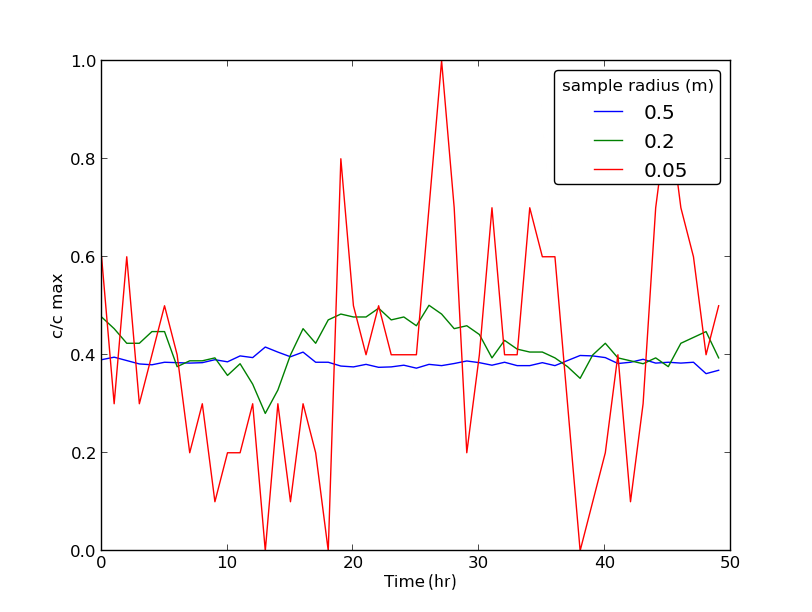
\includegraphics[width=3.2in]{../plots/newUse/concentrationOverTime.png} } }
      \caption{Temporal concentration profile for a single location.  The location is along the minor axis of the plume 6 m from the source.  The y-axis show the concentration normalized by the maximum concentration $(c/c_{max})$}
   \label{pic:overTime}
 \end{figure}

\begin{figure}[thpb]
      \centering
	\framebox{\parbox{3in}{
	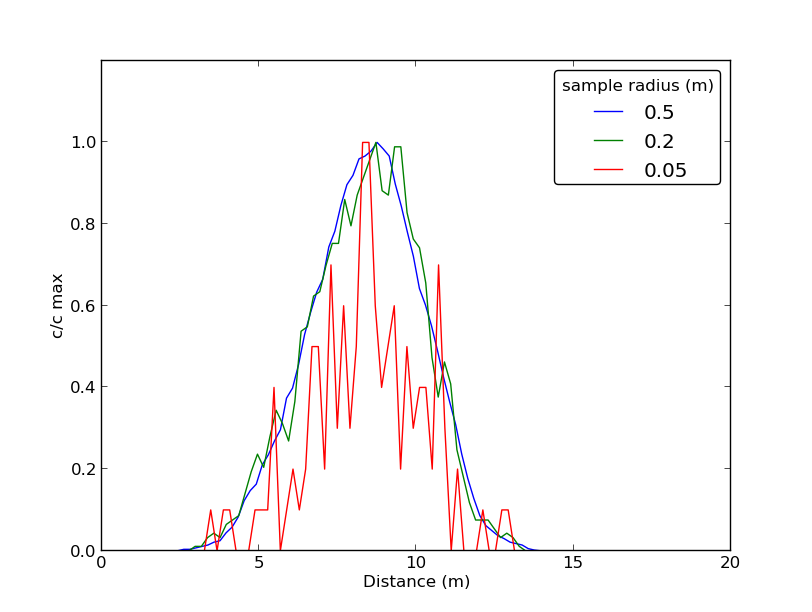
\includegraphics[width=3.2in]{../plots/newUse/concentrationOverSpace.png} } }
      \caption{Spatial variability of predicted concentration measurements as a function of the sampling radius model parameter.  the profile is generated for a line parallel to the minor axis of the plume 6 m from the source.  The y-axis show the concentration normalized by the maximum concentration $(c/c_{max})$}
   \label{pic:overSpace}
 \end{figure}

\begin{figure}[thpb]
      \centering
	\framebox{\parbox{3in}{
	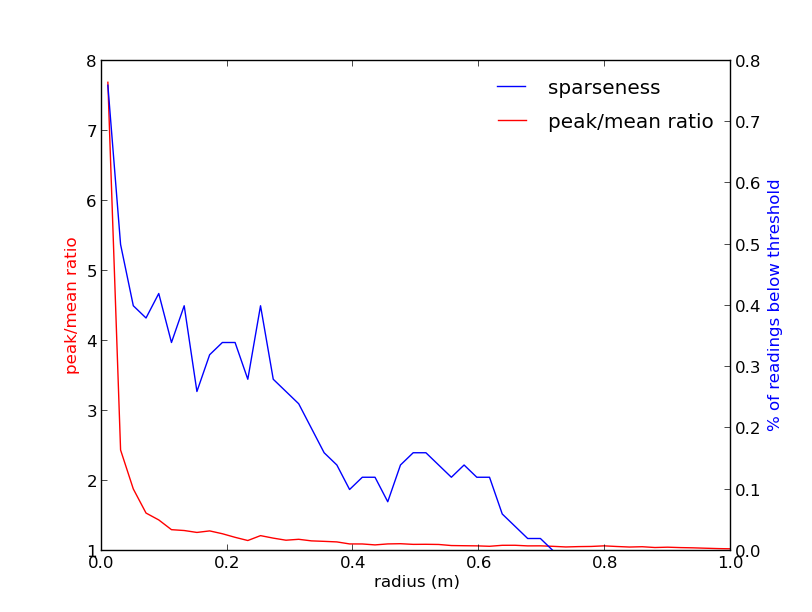
\includegraphics[width=3.2in]{../plots/newUse/sparsandP2mOverRadius.png} } }
      \caption{Sparsity and Peak/mean radius as a function of the sampling radius.   The peak/mean ratio values are shown on the right y-axis and the sparsity metric is shown on the left y-axis.}
   \label{pic:SandP2MoverRad}
 \end{figure}

Fig. \ref{pic:overTime} shows the concentration profile over time at a location downstream from the source of the plume.  When the sampling radius \unit[0.5]{m}, the concentration is nearly constant.  When the sampling radius is very low, 0.05 m, the concentration profile is very similar to how Jones and Crimaldi described the structure of an instantaneous plume \cite{Crimaldi2002}\cite{Jones1983}.  This graph shows that far from the limit the simulation represents metrics similar  to the  experimental sampling represented in Fig. \ref{pic:simSpont} suggesting that by varying the sampling radius the model can represent the variability one would expect from field robot experiments.

Fig. \ref{pic:overSpace} shows the spatial distribution of the plume concentration along the minor axis 6 m down stream from the source.    When the radius is at \unit[0.5]{m}, the concentration profile nearly follows a normal curve, like what we would expect in the limit. When the sampling radius is set to \unit[0.05]{m} the concentration profile is very irregular.  Though it generally follows a bell curve, it has a very large variation.  The middle line at \unit[0.2]{m} shows a point between the two extremes. 

Fig. \ref{pic:SandP2MoverRad} shows the sparsity and peak/mean ratio as the sampling radius moves from 0 to 1. This shows how tuning the radius effects the sparsity and the peak/mean ratio.  Additionally, by adjusting the threshold value, we can bring these two curves closer together.  

\section{Case Study}\label{part:caseStudy}
%<<<<<<< HEAD
To illustrate the utility of proposed environmental model we present the evaluation of the control algorithm developed in \cite{Li2014}.  The goal of the controller is to track the dynamic plume front based on concentration measurements made by mobile robots.  This control approach considers the local gradient, but also includes a transport model (advection and diffusion) in the estimation and control framework.  Previous work, using a simulated Gaussian plume environmental model (low variability), has shown the controller successfully tracks plume front movement at the water surface.  For this case-study we considered the single robot case, but the algorithm can be extended to multiple mobile robots using nearest-neighbor communication.  For the details of the controller implementation in the robotic simulation platform, please refer to our companion paper \cite{Fahad2015}.


% based and that this approach can be used for a single mobile robot as well as multiple robots with nearest-neighbor communication.  However, these results were based on a Gaussian implementation of the pollution environment, i.e., the simulated plume had low intermittancy. 

%To illustrate the use of the proposed model we implement the single robot control algorithm detailed in \cite{Li2014}.  We use the environmental model described above to emulate the temporal and spatial dynamics of a chemical plume having the same advection and diffusion characteristics as the Gaussian model used in \cite{Li2014}.  This allows us to evaluate the control algorithm in a scenario where the sensor observations necessary as input to the control algorithm are generated by the proposed model, enabling prediction of how the control algorithm will perform when exposed to the variability to be expected in sensor observations from a mobile robot operating in a coastal ocean environment. 

Two test cases are discussed below: the first with low variability (approximating the Gaussian plume) and the second with high variability (approximating the packet or filament concentration gradients observed in other ocean experiments).  For both cases, the control objective is to follow a particular concentration contour (specified as \unit[30]{\%} of the maximum expected concentration).  For both cases the underlying model parameters specifying advection and diffusion behavior are identical; the only difference between the two test cases is the value used for the model parameter that controls variability.
%=======
%To illustrate the utility of proposed environmental model we present the evaluation of the control algorithm developed in \cite{Li2014}.  The goal of the controller is to track the dynamic plume front based on concentration measurements made by mobile robotic robots.  The approach not only considers the local gradient, but also includes a transport model (advection and diffusion) in the estimation and control framework.  It has been shown in simulation that this approach can successfully track the movement of a plume front at the water surface based and that this approach can be used for a single mobile robot as well as multiple robots with nearest-neighbor communication.  However, these results were based on a Gaussian implementation of the pollution environment, i.e., the simulated plume had low intermittancy.  This case-study shows how we an use the proposed environmental model to capture the spatial and temporal variability associated with a the actual sensor observations of a mobile robot operating in a coastal ocean environment. 
%>>>>>>> 7493217211dda948adb86b697bfc2bf91054805e

%<<<<<<< HEAD
%For this illustration we present two test cases: the first with low variability (approximating the Gaussian plume) and the second with high variability (approximating the packetized or filament concentration gradients observed in other ocean experiments).  For both cases the goal of the controller is to follow the 0.3 line and the environmental factors (advection and diffusion coefficients) were identical.
%=======%
The results of the first case, low variability, are illustrated in Fig.~\ref{f:case1}.  For this case the concentration sampling radius of the environmental model is set to \unit[0.5]{m} to approximate the Gaussian plume model through introduction of spatial smoothing.  This value was chosen for the sampling radius because it produces a nearly smooth concentration curve, but still retains some variance.   The control strategy successfully guides the mobile robot in a path to follow the plume front by tracking the gradient contour. These results are consistent with the findings reported in \cite{Li2014} suggesting that the proposed model approximates the Gaussian plume model when the concentration sampling radius is sufficiently high.
%>>>>>>> da17ff319fe44b3353ec9faafff436919986704b

%<<<<<<< HEAD
%These results confirm that for this low variablity case the model approximates the Gaussian plume model used in the orginal evaluation of the algorithm by \cite{Li2014}.  
%=======
%The results of the first case, low variability, are illustrated in Fig.~\ref{pic:working}.  For this case the concentration sampling radius of the environmental model is set to \unit[0.5]{m} to approximate the Gaussian plume model.  The control strategy successfully guides the mobile robot in a path to follow the plume front by tracking the gradient contour. These results confirm that for this low variability case the model approximates the Gaussian plume model used in the original evaluation of the algorithm by \cite{Li2014}.  
%>>>>>>> 7493217211dda948adb86b697bfc2bf91054805e

%To test the usefulness of our model, we apply it to the control algorithm developed in \cite{Li2014}.  We run the controller using a concentration sampling radius of $0.5$ m and $0.05$ m.   The controller is set to follow the concentration line of $0.3$kg/L oil.   The two figures below show the results.  Each shows the plume and the history of the robots path along the plume, a plot of the history of the concentration readings while traveling along the plume, and a plot showing the path isolated from the plume for easy reading.  
%\begin{figure}[thpb]
   %   \centering
%	\framebox{\parbox{3in}{
%<<<<<<< HEAD
%	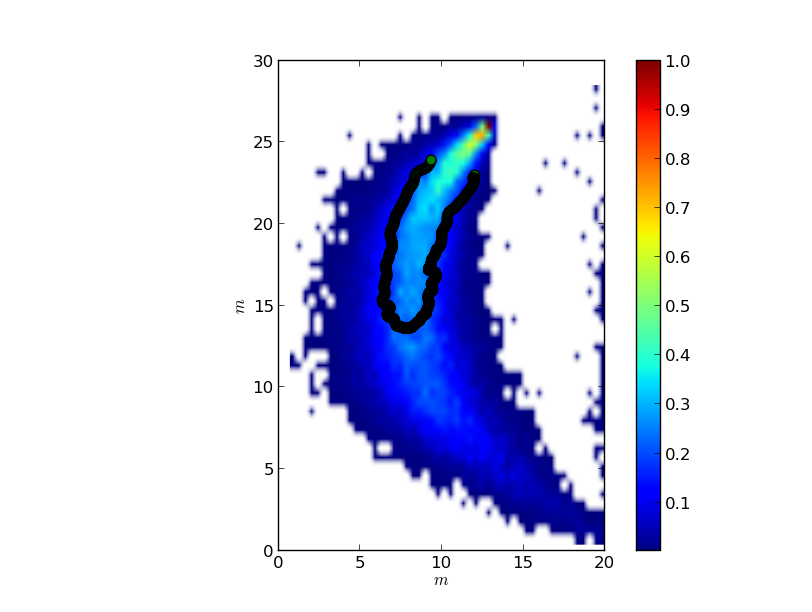
\includegraphics[width=3.2in]{../plots/inUse/mapSuccess.png} } }
   %   \caption{Plot of path of robot at 10 hours with a sample radius of 0.5 m}
  % \label{pic:workingPath}
 %\end{figure}

\begin{figure}[thpb]
      \centering
	\framebox{\parbox{3in}{
	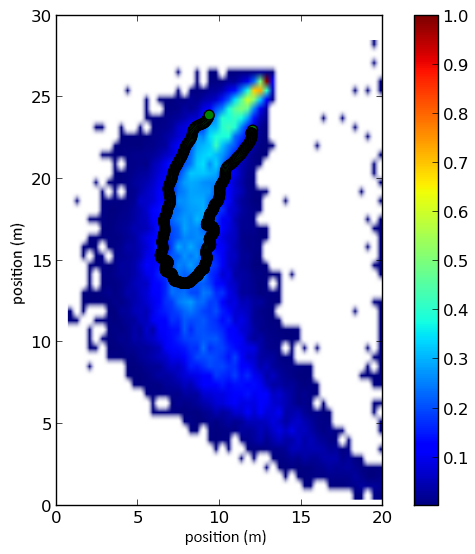
\includegraphics[width=2.6in]{../plots/newUse/mapSuccess.png}
	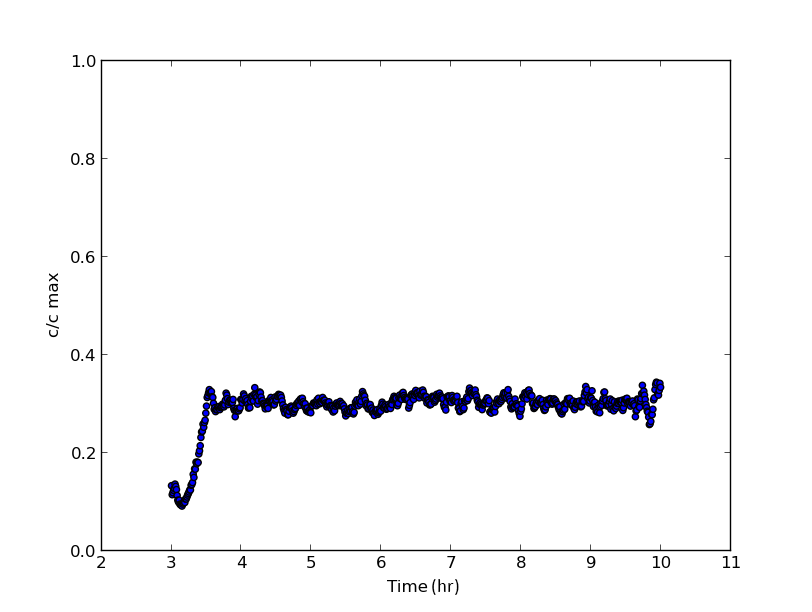
\includegraphics[width=3in]{../plots/newUse/concentrationSuccess.png} } }
          \caption{Results for the low variability test case for single robot tracking the plume front.  The upper image shows the chemical concentration of a pollution plume at the end of the simulation run.  The control objective for the mobile robot is to follow the 30\% contour.  The robot track is shown superimposed on the plume as a black line.  The lower graph shows the time history of the concentration observations made by the mobile platform.}
   \label{f:case1}
 \end{figure}

For the second case we introduce variability that we might anticipate when we transition the control algorithm to field implementation, i.e., testing the algorithms on mobile robots operating in a coastal ocean environment using on-board sensors to observe pollution concentration.  Based on previous experimental work we can expect significant variability in these instantaneous measurements.  To prepare for this transition from simulation to experiment it is necessary to evaluate how the control approach performs in a more authentic environmental scenario, not just in the idealized Gaussian plume case.   To accomplish this we reduce the concentration sampling radius to \unit[0.05]{m} which still captures the underlying advection and diffusion, but also emulates the intermittency and peak/mean ratio described by Jones and Crimaldi.  The results are shown in Fig.~\ref{f:case2}, which illustrates that the increased variability prevents the algorithm from guiding the robot to follow the plume front. The robot track shows that the robot moves very little from its original position, suggesting that the reliance on gradient measurements is brittle with respect to the localized, quickly varying concentration measurements typical of experimental implementation.  The concentration readings illustrate the intermittency we might expect from an on-board sensor where the concentration at any given point is likely to be zero because of the packetized pollution.  While this result shows that the original control algorithm is not robust to this intermittency, it does illustrate the capability of the environmental model we propose to capture this effect.  Furthermore we can vary a single parameter, the concentration sampling radius, to smoothly transition from the idealized Gaussian plume case to a more authentic case that captures the additional complexity of an intermittent plume environment observed in ocean experiments.
%=======
   %   \caption{Plot of path and concentration reading at 9 seconds with a sample radius of 0.5 m}
  % \label{pic:working}
% \end{figure}

%For the second case we introduce the variability that we might expect when we transition the control algorithm to a field experiment.  To accomplish this we reduce the concentration sampling radius to \unit[0.05]{m} which still captures the underlying advection and diffusion put simulates the intermittancy of the ocean environment.  The results of this case are shown in Fig.~\ref{pic:notworking}.  In this case the variability prevents the algorithm from guiding the robot to follow the plume front as evidenced by the robot track which shows that the robot moves very little from its original position.  The concentration readings are illustrate the itermittancy we might expect from an onboard sensor where the the concentration at any given point is likely to be zero because of the packets and filaments of pollution.  While this result shows that the original control algorithm is not robust to this intermittancy it does illustrate the capability of the environmental model we propose to capture this effect.  Furthermore we can vary a single parameter, the concentration sampling radius, to smoothly transition from the idealized Gaussian plume case to a more authentic case that captures the additional complexity of an intermittent plume environment observed in ocean experiments.
%>>>>>>> 7493217211dda948adb86b697bfc2bf91054805e

\begin{figure}[thpb]
      \centering
	\framebox{\parbox{3in}{
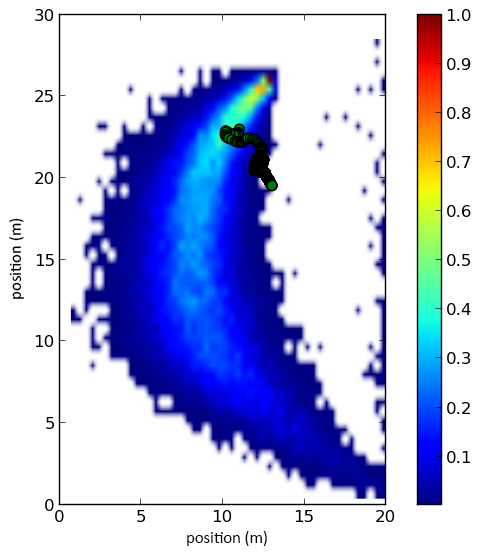
\includegraphics[width=2.6in]{../plots/newUse/mapNot.png}
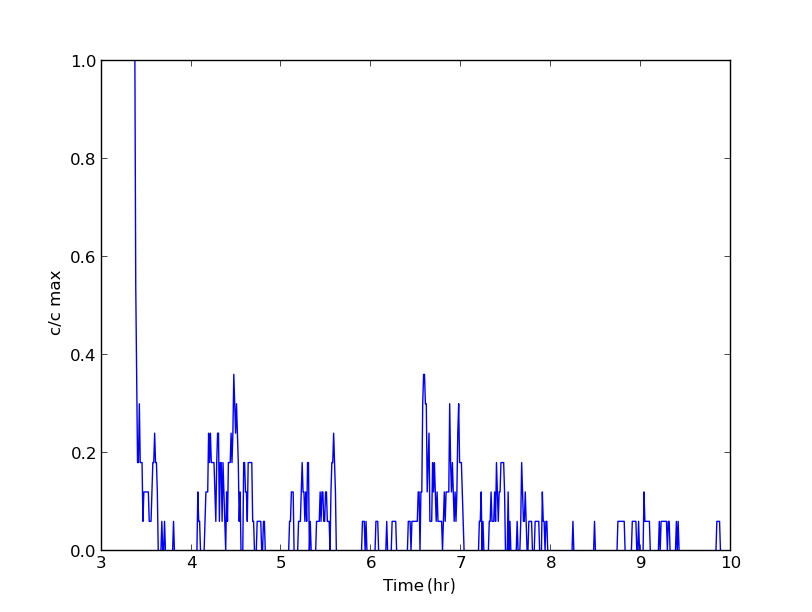
\includegraphics[width=3in]{../plots/newUse/concentrationNotLine.png}
	%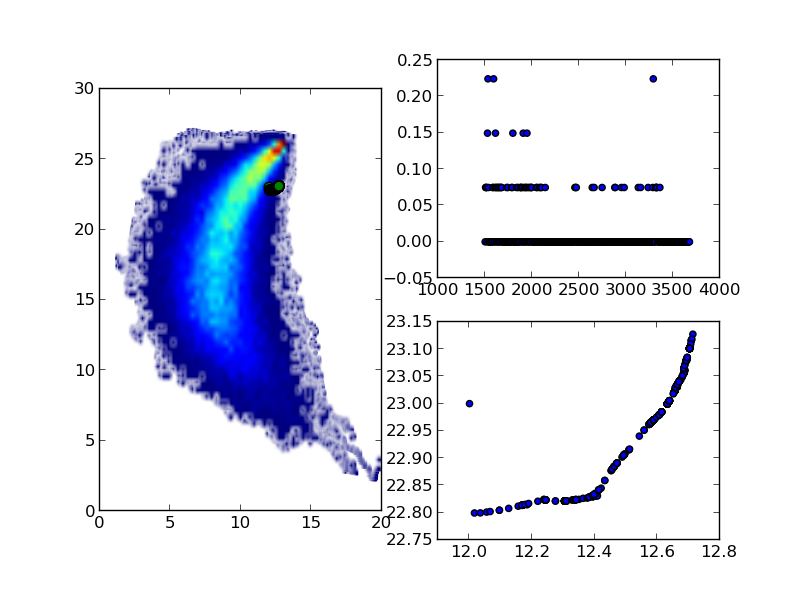
\includegraphics[width=3.2in]{../plots/inUse/_bad435.png} 
} }
%<<<<<<< HEAD
      \caption{Results for the high variability test case.  In the upper image the robot location is shown superimposed on the plume image.  The lower graph shows the time history the concentration observations made by the mobile platform, illustrating the variability in instantaneous observations.}
   \label{f:case2}
%=======
  %    \caption{Plot of path and concentration reading at 8 seconds with a sample raidus of 0.05 m}
  % \label{pic:notworking}
%>>>>>>> 7493217211dda948adb86b697bfc2bf91054805e
%>>>>>>> da17ff319fe44b3353ec9faafff436919986704b
 \end{figure}

%For the second case we introduce the variability that we might expect when we transition the control algorithm to a field experiment.  To accomplish this we reduce the concentration sampling radius to \unit[0.05]{m} which still captures the underlying advection and diffusion put simulates the intermittancy of the ocean environment.  The results of this case are shown in Fig.~\ref{pic:notworking}.  In this case the variability prevents the algorithm from guiding the robot to follow the plume front as evidenced by the robot track which shows that the robot moves very little from its original position.  The concentration readings are illustrate the itermittancy we might expect from an onboard sensor where the the concentration at any given point is likely to be zero because of the packets and filaments of pollution.  While this result shows that the original control algorithm is not robust to this intermittancy it does illustrate the capability of the environmental model we propose to capture this effect.  Furthermore we can vary a single parameter, the concentration sampling radius, to smoothly transition from the idealized Gaussian plume case to a more authentic case that captures the additional complexity of an intermittent plume environment observed in ocean experiments.

%\begin{figure}[thpb]
  %    \centering
%	\framebox{\parbox{3in}{
%	\includegraphics[width=3.2in]{../plots/inUse/mapFail.png} } }
   %   \caption{Plot of path and concentration reading at 8 seconds with a sample radius of 0.05 m}
 %  \label{pic:notworking}
 %\end{figure}


%\begin{figure}[thpb]
 %     \centering
%	\framebox{\parbox{3in}{
%	\includegraphics[width=3.2in]{../plots/inUse/concentrationFail.png} } }
 %     \caption{Plot of path and concentration reading at 8 seconds with a sample raidus of 0.05 m}
  % \label{pic:notworking}
% \end{figure}
%When the sampling radius is set to $0.5$ m, the robot seems successful.  It follows the edge of the plume, though does so much slower than the results in Shuai's simulation \cite{Li2014}.  Still, the robot behaves very similarly to how it was designed to on the Gaussian plume.  We see  it very nearly follows the desired line. 

% When the sampling radius is set to $0.05$ m, we see that the concentration readings are wildly sporadic, with the majority of them reading $0$.  Because of this, the robot moves very little, and mostly back and forth.  The readings are so sporadic and variant that the robot does not know how to respond.    

%This shows that while the controller will work for plumes that are slightly   


\section{Conclusions}\label{part:conclusion}
We present an environmental model of pollution plumes in an ocean environment.  In addition to the underlying advection and diffusion dynamics, the model explicitly represents variability and intermittency in pollution concentration measurements to enable evaluation of robotic control algorithms.  The parametric representation allows the evaluation of control algorithm robustness with respect to variability.  To successfully transition algorithms developed in simulation it is critical to understand how these algorithms will perform with the intermittent sensor measurements to be expected in field deployments.
 
We illustrated the utility of this approach through a case-study.  In this case-study we evaluated the performance of a previously proposed control algorithm using the proposed environmental model.  We showed that with the variability set sufficiently low, by increasing the size of the concentration sampling radius, the model approximates the Gaussian plume model.  As variability is increased the performance of the control algorithm degrades.  Understanding the relationship between variability and performance is critical to transitioning these algorithms into the field.

Field experiments in marine environments are costly and time consuming, therefore it is critical that the simulations used to evaluate their efficacy capture the salient aspects of ocean operations.  Previous research has shown that the real-time sensor observations of pollution plumes in such environments are highly variable; to be experimentally successful robotic control algorithms must address concentration intermittency. The model we propose provides a method for emulating this intermittency to quantify performance of candidate robotic algorithms tasked with supporting ocean pollution remediation.  In application ocean pollution dynamics have a wide variety of characteristics.  As researchers transition robotic algorithms to work in such environments it is important to predict how these strategies will perform when implemented on operational hardware.  The proposed model allows developers to evaluate the performance in a wide variety of test cases to better quantify sensitivity to variability in sensor measurements before incurring the costs associated with experimental deployment.

%This paper presents a model for oil spills suitable for the development of robotic command and control algorithms.  This model can be tuned to represent the theoretical and idealized image of a plume, and can also represent the extreme characteristics that in an instantaneous plume.  By developing and testing control algorithms on a continuous variation of models, control algorithm developers can create a more robust controller.  Many control algorithms are developed for situations that are very specific and are then tested in simulation on these very specific situation.  In application, an oil spill can have a wide range of characteristics.  It is important to know which conditions and kinds of plumes the controller will work for.  This simulation allows developers to test controllers on many varying know under which conditions and which kinds of plumes the controller will function. 

%%%%%%%%%%%%%%%%%%%%%%%%%%%%%%%%%%%%%%%%%%%%%%%%%%%%%
%%%%%%%%%%%%%%%%%%%%%%%%%%%%%%%%%%%%%%%%%%%%%%%%%%%%%

\section*{Acknowledgments}
This material is based upon work supported by the National Science Foundation under Grants IIS-1217659 (Saul, Marriott, and Bingham) and IIS-1218155 (Fahad and Guo).


\bibliography{plumeICRA_2015.bib}{}
\bibliographystyle{plain}


%%%%%%%%%%%%%%%%%%%%%%%%%%%%%%%%%%%%%%%%%%%%%%%%%%%%%
%%%%%%%%%%%%%%%%%%%%%%%%%%%%%%%%%%%%%%%%%%%%%%%%%%%%%




\end{document}
